\documentclass[notheorems]{beamer}

\usepackage{amsmath}
\usepackage{amssymb}
\usepackage[scale=2]{ccicons}
\usepackage{appendixnumberbeamer}
\usepackage{booktabs}
\usepackage[toc,page]{appendix}
\usepackage{graphicx}
\usepackage{xspace}
\usepackage{adjustbox, lipsum}
\usepackage{bbm}
\usepackage{algorithm}
\usepackage{algpseudocode}

%tikz stuff
\usepackage{caption}
\usepackage{subcaption}
\usepackage{tikz}
\usepackage{mathdots}
\usepackage{yhmath}
\usepackage{cancel}
\usepackage{color}
\usepackage{siunitx}
\usepackage{array}
\usepackage{multirow}
\usepackage{amssymb}
\usepackage{gensymb}
\usepackage{tabularx}
\usetikzlibrary{fadings}

\input{macros/math}

% absolute positioning
\usepackage[absolute,overlay]{textpos}

\newcommand{\source}[1]{{\let\thefootnote\relax\footnote{{\tiny #1}}}}


\setbeamertemplate{frametitle}
  {\insertframetitle\strut%
    \vskip0\baselineskip%
    \leaders\vrule width \textwidth\vskip0.4pt%
    \vskip0pt%
    \nointerlineskip}
\setbeamertemplate{itemize item}{$\bullet$}
\setbeamertemplate{navigation symbols}{}
\setbeamertemplate{footline}[text line]{%
    \hfill\strut{%
        \scriptsize\sf\color{black!60}%
        \quad\insertframenumber/\inserttotalframenumber
    }%
    \hfill%
}

\AtBeginSection[]{
{ \setbeamercolor{background canvas}{bg=LightCharcoal}
  \begin{frame}
  \vfill
  \centering
  \begin{beamercolorbox}[sep=8pt,center,shadow=true,rounded=true]{title}
    \usebeamerfont{title} \insertsectionhead\par%
  \end{beamercolorbox}
  \vfill
  \end{frame}
}}

\setbeamerfont{bibliography item}{size=\footnotesize}
\setbeamerfont{bibliography entry author}{size=\footnotesize}
\setbeamerfont{bibliography entry title}{size=\footnotesize}
\setbeamerfont{bibliography entry location}{size=\footnotesize}
\setbeamerfont{bibliography entry note}{size=\footnotesize}

% Define some colors:
\definecolor{DarkFern}{HTML}{407428}
\definecolor{DarkCharcoal}{HTML}{4D4944}
\colorlet{Fern}{DarkFern!85!white}
\colorlet{Charcoal}{DarkCharcoal!85!white}
\colorlet{LightCharcoal}{Charcoal!50!white}
\colorlet{AlertColor}{orange!80!black}
\colorlet{DarkRed}{red!70!black}
\colorlet{DarkBlue}{blue!70!black}
\colorlet{DarkGreen}{green!70!black}
% Use the colors:
\setbeamercolor{title}{fg=DarkBlue}
\setbeamercolor{frametitle}{fg=DarkBlue}
\setbeamercolor{normal text}{fg=black}
\setbeamercolor{block title}{fg=black,bg=Fern!25!white}
\setbeamercolor{block body}{fg=black,bg=Fern!25!white}
\setbeamercolor{alerted text}{fg=AlertColor}
\setbeamercolor{itemize item}{fg=DarkCharcoal}

%Information to be included in the title page:
\title{Why Does Deep Learning Work?}

\author{Aaron Mishkin}
\institute{UBC MLRG 2019W1}
\date{}

% Outline:
    % 1) Motivation and Intro: Success of Deep Learning
        % i)    Image Classification and Localization
        % ii)   NLP and Speech
        % iii)  Generative modeling (GANs and VAEs)
    % 2) Traditional Theory: Model Capacity and Generalization
    % 3) Perceptron: An Instructive Example
        % i)    Mistake Bound
        % ii)   1st Generalization Bound
        % iii)  2nd Generalization Bound
        % iv)   Observations: Dimension Independence and Role of Optimization
    % 4) Failure of the Current Theory.
    % 5) Recent Areas of Research:
        % i)    Types of Minima
        % ii)   Properties of Optimizers
        % iii)  Over-Parameterization

\begin{document}

    \begin{frame}

        \titlepage

    \end{frame}

    \begin{frame}{Why Does Deep Learning Work?}

        {\Large \centering Common refrains from deep learning: \vspace{0.75cm} }

        \begin{itemize} \large
            \item ``Always make your neural network \textbf{as big as possible}!''\vspace{0.25cm}
            \item ``Neural networks \textbf{generalize} because they're trained with \textbf{stochastic gradient descent (SGD)}.''\vspace{0.25cm}
            \item ``\textbf{Sharp minima} are bad and \textbf{shallow} minima are good.'' \vspace{0.25cm}
            \item ``\textbf{SGD} finds \textbf{flat} local minima.''
        \end{itemize}

        {\Large \vspace{1.25cm} \centering Where do these ideas come from? \vspace{1cm} }

    \end{frame}

    \section{Deep Learning Works!}

    \begin{frame}{Deep Learning Works: Object Localization}

        \begin{figure}
            \centering
            \begin{subfigure}[c]{0.45\textwidth}
                \includegraphics[width=\linewidth]{figures/bounding_boxes}
            \end{subfigure}
            \begin{subfigure}[t]{0.45\textwidth}
                \includegraphics[width=\textwidth]{figures/region_based_cnn}
            \end{subfigure}
        \end{figure}

        \begin{textblock*}{5cm}(7cm,5.75cm) % {block width} (coords)
           Object localization with Fast R-CNNs \cite{girshick2015fast}.
        \end{textblock*}

        \source{https://arxiv.org/abs/1707.07012}
        \source{https://towardsdatascience.com/deep-learning-for-object-detection-a-comprehensive-review-73930816d8d9}
    \end{frame}

    \begin{frame}{Deep Learning Works: Image Segmentation}

        Image segmentation using fully convolutional networks \cite{long2015fully}.

        \begin{figure}
            \centering
            \includegraphics[width=0.6\textwidth]{figures/alex-model}
        \end{figure}
        \vspace{-0.5cm}
        \begin{figure}
            \centering
            \scalebox{1}{
                \begin{tabular}{c c | c c | c c}
                    \includegraphics[width=0.125\linewidth]{figures/semantic_segmentation/vis/img/000008_image.png} &
                    \includegraphics[width=0.125\linewidth]{figures/semantic_segmentation/vis/prediction/000008_prediction.png} &

                    \includegraphics[width=0.125\linewidth]{figures/semantic_segmentation/vis/img/000046_image.png} &
                    \includegraphics[width=0.125\linewidth]{figures/semantic_segmentation/vis/prediction/000046_prediction.png} &

                    \includegraphics[width=0.125\linewidth]{figures/semantic_segmentation/vis/img/000087_image.png} &
                    \includegraphics[width=0.125\linewidth]{figures/semantic_segmentation/vis/prediction/000087_prediction.png} \\

                    \includegraphics[width=0.125\linewidth]{figures/semantic_segmentation/vis/img/000131_image.png} &
                    \includegraphics[width=0.125\linewidth]{figures/semantic_segmentation/vis/prediction/000131_prediction.png} &

                    \includegraphics[width=0.125\linewidth]{figures/semantic_segmentation/vis/img/000195_image.png} &
                    \includegraphics[width=0.125\linewidth]{figures/semantic_segmentation/vis/prediction/000195_prediction.png} &

                    \includegraphics[width=0.125\linewidth]{figures/semantic_segmentation/vis/img/000199_image.png} &
                    \includegraphics[width=0.125\linewidth]{figures/semantic_segmentation/vis/prediction/000199_prediction.png} \\

                \end{tabular}
            }
        \end{figure}

        \source{https://arxiv.org/abs/1411.4038}
        \source{https://arxiv.org/abs/1802.02611}

    \end{frame}

    \begin{frame}{Deep Learning Works: Machine Translation (1) }

        \begin{figure}
            \includegraphics[width=0.98\textwidth]{figures/google_translate}
        \end{figure}
        Google's Neural Machine Translation System:
        \begin{itemize}
            \item consists of a \textbf{deep LSTM network} with 8 encoder and 8 decoder layers using attention and residual connections.
            \item reduced translation errors ``by an average of \textbf{60\%} compared to Google's phrase-based'' system.
        \end{itemize}

    \end{frame}

    \begin{frame}{Deep Learning Works: Machine Translation (2) }

        \begin{figure}
            \begin{minipage}[t]{.42\textwidth}
                \includegraphics[width=\textwidth]{figures/translate_image}
             \end{minipage} %
             \hfill%
            \begin{minipage}{.42\textwidth}
                \vspace{-7.3cm}
                {\footnotesize Berlin POLIZEI BERLIN The Berlin police informs about burglary protection On Thursday, 23rd May 2019, between 3:00 pm and 6:00 pm, police officers hold an information event on burglary protection in their residential area. In the process, the police will visit residential buildings and shops and inform you directly about security options. At the same time, police officers at an information stand in the Hagelberger Str. 34, 10965 Berlin show them, with the help of window and door models, how they can effectively secure their property...}
            \end{minipage}
        \end{figure}
    \end{frame}

    \begin{frame}{Deep Learning Works: Generative Models}

        \begin{center}
            StyleGAN: image generatation with hierarchical style transfer \cite{karras2019style}.
        \end{center}

        \begin{figure}
            \centering
            \includegraphics[width=0.7\textwidth]{figures/style_transfer}
        \end{figure}

        \source{https://arxiv.org/abs/1812.04948}
    \end{frame}


    \begin{frame}{Deep Learning Works: Model Sizes (1)}
        \begin{center}
            \textbf{Accuracy on ImageNet} (2012 ILSVRC)
        \end{center}
        \begin{figure}
            \centering
            \includegraphics[width=0.7\linewidth]{figures/FLOPS1}
        \end{figure}

        \source{https://arxiv.org/abs/1810.00736}

    \end{frame}

    \begin{frame}{Deep Learning Works: Model Sizes (2)}

        \textbf{Accuracy on ImageNet} (2012 ILSVRC): Exponentially more parameters are needed to improve accuracy.
        \begin{figure}
            \centering
            \includegraphics[width=0.85\textwidth]{figures/Params-Diagram-SE}
        \end{figure}

        \source{https://arxiv.org/abs/1707.07012}

    \end{frame}

    \begin{frame}{Deep Learning Works: Bias-Variance}

        {\Large But what about the \textbf{bias-variance} trade-off?}\\
        \vspace{0.75cm}

        Let $y = f(x) + \epsilon$, where $\epsilon \sim \mathcal{N}(0, \sigma^2)$,

        \[ \E \sbr{ \rbr{y - \hat f(x)}^2 } = \textbf{Bias}\sbr{\hat f(x)}^2 + \textbf{Var}\sbr{\hat f(x)} + \sigma^2 \]

        \begin{figure}
            \includegraphics[width=0.7\textwidth]{figures/bias_variance}
        \end{figure}

        \source{http://scott.fortmann-roe.com/docs/BiasVariance.html}

    \end{frame}

    \begin{frame}{Bias-Variance: Deep Models}

        We expect bigger architectures to:
        \begin{itemize}
            \item have \textbf{lower bias} because have they more parameters,
            \item but \textbf{higher variance} across different training sets.
        \end{itemize}
        \vspace{0.1cm}
        \begin{minipage}[c]{0.68\textwidth}
            \begin{figure}
                \includegraphics[width=\textwidth]{figures/Params-Diagram-SE}%
            \end{figure}
        \end{minipage}%
        \hfill%
        \begin{minipage}[c]{0.28\textwidth}
            \centering
            \Large Shouldn't we see this in action with deep models?
        \end{minipage}
        \source{https://arxiv.org/abs/1707.07012}
    \end{frame}

    \begin{frame}{Bias-Variance: Optimization Bias}

        Maybe we're \textbf{overfitting} architectures to the test set!

        \begin{figure}
            \centering
            \begin{subfigure}{0.48\textwidth}
                \includegraphics[width=\linewidth]{figures/intro_plot_cifar10_without_legend.pdf}
            \end{subfigure}
            \hfill
            \begin{subfigure}{0.48\textwidth}
                \includegraphics[width=\linewidth]{figures/intro_plot_imagenet_without_legend.pdf}
            \end{subfigure}
            \begin{subfigure}{\textwidth}
                \vspace{-.15cm}
                \centering
                \includegraphics[width=.75\linewidth]{figures/intro_plot_separate_legend_horizontal.pdf}
            \end{subfigure}
        \end{figure}

        New Test Sets for CIFAR-10 and ImageNet~\cite{recht2019imagenet}:
        \begin{itemize}
            \item ``the relative order of models is almost \textbf{exactly preserved}''
            \item ``there are \textbf{no diminishing returns} in accuracy''
        \end{itemize}

        \source{https://arxiv.org/abs/1902.10811}
    \end{frame}

    \begin{frame}{Bias-Variance: What's Happening?}
        \begin{center}
            {\huge Why do bigger neural networks lead to better accurracy? \vspace{1cm}\\ }

            {\huge The issue is how we think about model ``capacity''. \vspace{1cm}\\ }
        \end{center}


    \end{frame}

    \section{Perceptron: An Instructive Example}

    \begin{frame}{Learning Theory: A Brief Introduction}
        \textbf{Statistical learning theory} tries to develop guarantees for the performance of machine learning models.\vspace{0.5cm}\\
        \begin{itemize}
            \item Let $\mathcal{D} = \cbr{(x_i, y_i)}_{i=1}^n$ be a \textbf{training set} of input-output pairs.
                \begin{itemize}
                    \item $\mathcal{D}$ is formed by sampling $(x,y) \sim p(x,y)$ $n$ times.
                \end{itemize}
            \item Let $\mathcal{H}$ be a \textbf{hypothesis class}.
                \begin{itemize}
                    \item $\mathcal{H}$ is a fixed set of prediction functions $f(x) = \hat y$ that we pre-select.
                    \item $\mathcal{H}$ could be SVMs with RBF kernels, one-layer neural networks, etc.
                \end{itemize}
            \item A \textbf{learning algorithm} takes $\mathcal{D}$ as input and returns $\hat f \in \mathcal{H}$.
        \end{itemize}

        \vspace{0.5cm} What does it mean to \textbf{generalize} in this framework?

    \end{frame}

    \begin{frame}{Learning Theory: Risk and ERM}
        Let $\mathcal{L}$ be a loss function. We care about the \textbf{risk},
        \[ R(f) = \E_{p(x,y)} \sbr{\mathcal{L}(f(x), y)}. \]
        We don't know $p(x,y)$, but we do have the training set $\mathcal{D}$. The \textbf{empirical risk} is simply the loss on $\mathcal{D}$,
        \[ R_{\mathcal{D}}(f) = \frac{1}{n} \sum_{i=1}^n \mathcal{L}(f(x_i), y_i). \]
        \textbf{Empirical risk minimization (ERM)} is the learning algorithm
        \[ \hat f \; = \min_{f \in \mathcal{H}} R_{\mathcal{D}}(f) = \min_{f \in \mathcal{H}} \; \frac{1}{n} \sum_{i=1}^n \mathcal{L}(f(x_i), y_i). \]
        This is simple -- choose $\hat f$ to minimize the training loss.

    \end{frame}

    \begin{frame}{Perceptron: Definition}
        \textbf{Perceptron} is an early linear model for binary classification.
        \begin{itemize}
            \item Let $x \in \R^d$ and $y \in \cbr{-1,1}$.
            \item $\mathcal{H}$ is the set of hyper-planes defined by $w \in \R^d$.
            \item Given weight vector $w$, $f_w(x) = \text{sign}(\langle w, x \rangle)$.
        \end{itemize}
        \textbf{Perceptron} is a neural network with one unit and sign activation.
        \begin{figure}
            \includegraphics[width=0.6\textwidth]{figures/perceptron}
        \end{figure}

        \source{https://www.javatpoint.com/pytorch-perceptron}

    \end{frame}

    \begin{frame}{Perceptron: Learning Algorithm}
        \vspace{-0.5cm}
        \begin{center}
            \textbf{Perceptron} works by iteratively correcting its mistakes.
        \end{center}
        \vspace{-0.25cm}
        \begin{minipage}[t]{0.55\textwidth}
            \begin{algorithm}[H]
                \centering
                \caption{Perceptron Algorithm}
                \begin{algorithmic}[1]
                    \State $w_0 \gets 0$
                    \For{$t = 0 \dots N-1$}
                    \State select $(x_t, y_t) \in \mathcal{D}$
                        \If {$\text{sign}(\langle w_{t}, x_t \rangle) \neq y_t$}
                            \State $w_{t+1} \gets w_{t} + y_t x_t$
                        \Else
                            \State $w_{t+1} \gets w_{t}$
                        \EndIf
                    \EndFor
                \State \Return $w_{N}$
                \end{algorithmic}
                \label{alg:slang}
            \end{algorithm}
        \end{minipage}%
        \hfill%
        \begin{minipage}[t]{0.4\textwidth}
            \vspace{0.75cm}
            \begin{figure}
                \centering
                \includegraphics[width=1.2\textwidth]{figures/Perceptron_example}
            \end{figure}
        \end{minipage}

        \source{https://commons.wikimedia.org/wiki/File:Perceptron\_example.svg}
    \end{frame}

    \begin{frame}{Perceptron: Mistake Bound}
        \begin{theorem}[Perceptron Mistake Bound]
            We need two assumptions for perceptron to work:
            \begin{itemize}
                \item the data is \textbf{linearly separable} with margin $\gamma$.
                \item the input features have \textbf{bounded norm}: $\norm{x}_2 \leq R \; \forall x$
            \end{itemize}
            Then perceptron makes at most $R^2 / \gamma^2$ mistakes during training:
            \begin{minipage}[t]{0.6\textwidth}
                \[ \sum_{t=0}^{N-1} \mathbbm{1}\rbr{\text{sign}\langle w_t, x_t \rangle) \neq y_t} \leq \frac{R^2}{\gamma^2}. \]
                See bonus slides for proof.
            \end{minipage}
            \begin{minipage}[t]{0.35\textwidth}
                \vspace{0.2cm}
                \begin{figure}
                    \raggedleft
                    

\tikzset{every picture/.style={line width=0.75pt}} %set default line width to 0.75pt

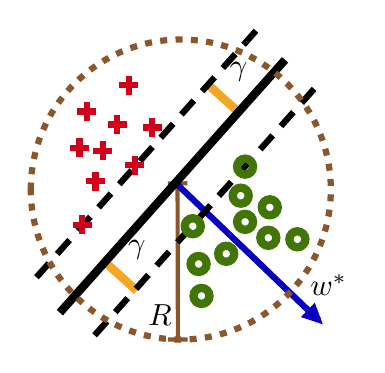
\begin{tikzpicture}[x=0.75pt,y=0.75pt,yscale=-0.7,xscale=0.7]
%uncomment if require: \path (0,346); %set diagram left start at 0, and has height of 346

%Straight Lines [id:da0330897325129611]
\draw [color={rgb, 255:red, 139; green, 87; blue, 42 }  ,draw opacity=1 ][line width=1.5]    (259,172) -- (259.25,279.5) ;
\draw [shift={(259.25,279.5)}, rotate = 269.87] [color={rgb, 255:red, 139; green, 87; blue, 42 }  ,draw opacity=1 ][line width=1.5]    (0,6.71) -- (0,-6.71)   ;
\draw [shift={(259,172)}, rotate = 269.87] [color={rgb, 255:red, 139; green, 87; blue, 42 }  ,draw opacity=1 ][line width=1.5]    (0,6.71) -- (0,-6.71)   ;
%Straight Lines [id:da41149837283513824]
\draw [color={rgb, 255:red, 8; green, 0; blue, 190 }  ,draw opacity=1 ][line width=2.25]    (257,171) -- (356.12,266.23) ;
\draw [shift={(359,269)}, rotate = 223.85] [fill={rgb, 255:red, 8; green, 0; blue, 190 }  ,fill opacity=1 ][line width=2.25]  [draw opacity=0] (14.29,-6.86) -- (0,0) -- (14.29,6.86) -- cycle    ;

%Straight Lines [id:da9187886013718665]
\draw [color={rgb, 255:red, 245; green, 166; blue, 35 }  ,draw opacity=1 ][line width=1.5]    (281.01,102.89) -- (302.01,121.89)(278.99,105.11) -- (299.99,124.11) ;


%Straight Lines [id:da7638090308640231]
\draw [color={rgb, 255:red, 245; green, 166; blue, 35 }  ,draw opacity=1 ][line width=1.5]    (211.01,225.89) -- (232.01,244.89)(208.99,228.11) -- (229.99,247.11) ;


%Straight Lines [id:da7725940690519442]
\draw [line width=2.25]  [dash pattern={on 6.75pt off 4.5pt}]  (353,107) -- (198,281) ;


%Straight Lines [id:da47426778305518247]
\draw [line width=2.25]  [dash pattern={on 6.75pt off 4.5pt}]  (313,67) -- (158,241) ;


%Shape: Circle [id:dp12477586784289807]
\draw  [color={rgb, 255:red, 65; green, 117; blue, 5 }  ,draw opacity=1 ][line width=3]  (264,201.5) .. controls (264,198.46) and (266.46,196) .. (269.5,196) .. controls (272.54,196) and (275,198.46) .. (275,201.5) .. controls (275,204.54) and (272.54,207) .. (269.5,207) .. controls (266.46,207) and (264,204.54) .. (264,201.5) -- cycle ;
%Shape: Circle [id:dp4467494249402495]
\draw  [color={rgb, 255:red, 65; green, 117; blue, 5 }  ,draw opacity=1 ][line width=3]  (300,160.5) .. controls (300,157.46) and (302.46,155) .. (305.5,155) .. controls (308.54,155) and (311,157.46) .. (311,160.5) .. controls (311,163.54) and (308.54,166) .. (305.5,166) .. controls (302.46,166) and (300,163.54) .. (300,160.5) -- cycle ;
\draw  [color={rgb, 255:red, 208; green, 2; blue, 27 }  ,draw opacity=1 ][fill={rgb, 255:red, 255; green, 0; blue, 0 }  ,fill opacity=1 ][line width=2.25]  (187,200.5) -- (200,200.5)(193.5,194) -- (193.5,207) ;
\draw  [color={rgb, 255:red, 208; green, 2; blue, 27 }  ,draw opacity=1 ][fill={rgb, 255:red, 255; green, 0; blue, 0 }  ,fill opacity=1 ][line width=2.25]  (185,147.5) -- (198,147.5)(191.5,141) -- (191.5,154) ;
\draw  [color={rgb, 255:red, 208; green, 2; blue, 27 }  ,draw opacity=1 ][fill={rgb, 255:red, 255; green, 0; blue, 0 }  ,fill opacity=1 ][line width=2.25]  (196,170.5) -- (209,170.5)(202.5,164) -- (202.5,177) ;
\draw  [color={rgb, 255:red, 208; green, 2; blue, 27 }  ,draw opacity=1 ][fill={rgb, 255:red, 255; green, 0; blue, 0 }  ,fill opacity=1 ][line width=2.25]  (223,159.5) -- (236,159.5)(229.5,153) -- (229.5,166) ;
\draw  [color={rgb, 255:red, 208; green, 2; blue, 27 }  ,draw opacity=1 ][fill={rgb, 255:red, 255; green, 0; blue, 0 }  ,fill opacity=1 ][line width=2.25]  (211,131.5) -- (224,131.5)(217.5,125) -- (217.5,138) ;
\draw  [color={rgb, 255:red, 208; green, 2; blue, 27 }  ,draw opacity=1 ][fill={rgb, 255:red, 255; green, 0; blue, 0 }  ,fill opacity=1 ][line width=2.25]  (201,149.5) -- (214,149.5)(207.5,143) -- (207.5,156) ;
\draw  [color={rgb, 255:red, 208; green, 2; blue, 27 }  ,draw opacity=1 ][fill={rgb, 255:red, 255; green, 0; blue, 0 }  ,fill opacity=1 ][line width=2.25]  (190,122.5) -- (203,122.5)(196.5,116) -- (196.5,129) ;
\draw  [color={rgb, 255:red, 208; green, 2; blue, 27 }  ,draw opacity=1 ][fill={rgb, 255:red, 255; green, 0; blue, 0 }  ,fill opacity=1 ][line width=2.25]  (235,133.5) -- (248,133.5)(241.5,127) -- (241.5,140) ;
%Straight Lines [id:da5998610493967904]
\draw [color={rgb, 255:red, 0; green, 0; blue, 0 }  ,draw opacity=1 ][line width=3]    (333,87) -- (178,261) ;


\draw  [color={rgb, 255:red, 208; green, 2; blue, 27 }  ,draw opacity=1 ][fill={rgb, 255:red, 255; green, 0; blue, 0 }  ,fill opacity=1 ][line width=2.25]  (219,104.5) -- (232,104.5)(225.5,98) -- (225.5,111) ;
%Shape: Circle [id:dp430217692111732]
\draw  [color={rgb, 255:red, 65; green, 117; blue, 5 }  ,draw opacity=1 ][line width=3]  (270,249.5) .. controls (270,246.46) and (272.46,244) .. (275.5,244) .. controls (278.54,244) and (281,246.46) .. (281,249.5) .. controls (281,252.54) and (278.54,255) .. (275.5,255) .. controls (272.46,255) and (270,252.54) .. (270,249.5) -- cycle ;
%Shape: Circle [id:dp03599857712709276]
\draw  [color={rgb, 255:red, 65; green, 117; blue, 5 }  ,draw opacity=1 ][line width=3]  (287,220.5) .. controls (287,217.46) and (289.46,215) .. (292.5,215) .. controls (295.54,215) and (298,217.46) .. (298,220.5) .. controls (298,223.54) and (295.54,226) .. (292.5,226) .. controls (289.46,226) and (287,223.54) .. (287,220.5) -- cycle ;
%Shape: Circle [id:dp7089060570275205]
\draw  [color={rgb, 255:red, 65; green, 117; blue, 5 }  ,draw opacity=1 ][line width=3]  (300,198.5) .. controls (300,195.46) and (302.46,193) .. (305.5,193) .. controls (308.54,193) and (311,195.46) .. (311,198.5) .. controls (311,201.54) and (308.54,204) .. (305.5,204) .. controls (302.46,204) and (300,201.54) .. (300,198.5) -- cycle ;
%Shape: Circle [id:dp6588880811889362]
\draw  [color={rgb, 255:red, 65; green, 117; blue, 5 }  ,draw opacity=1 ][line width=3]  (317,188.5) .. controls (317,185.46) and (319.46,183) .. (322.5,183) .. controls (325.54,183) and (328,185.46) .. (328,188.5) .. controls (328,191.54) and (325.54,194) .. (322.5,194) .. controls (319.46,194) and (317,191.54) .. (317,188.5) -- cycle ;
%Shape: Circle [id:dp042625042794921075]
\draw  [color={rgb, 255:red, 65; green, 117; blue, 5 }  ,draw opacity=1 ][line width=3]  (268,227.5) .. controls (268,224.46) and (270.46,222) .. (273.5,222) .. controls (276.54,222) and (279,224.46) .. (279,227.5) .. controls (279,230.54) and (276.54,233) .. (273.5,233) .. controls (270.46,233) and (268,230.54) .. (268,227.5) -- cycle ;
%Shape: Circle [id:dp2175111334914439]
\draw  [color={rgb, 255:red, 65; green, 117; blue, 5 }  ,draw opacity=1 ][line width=3]  (297,180.5) .. controls (297,177.46) and (299.46,175) .. (302.5,175) .. controls (305.54,175) and (308,177.46) .. (308,180.5) .. controls (308,183.54) and (305.54,186) .. (302.5,186) .. controls (299.46,186) and (297,183.54) .. (297,180.5) -- cycle ;
%Shape: Circle [id:dp2565384713500847]
\draw  [color={rgb, 255:red, 65; green, 117; blue, 5 }  ,draw opacity=1 ][line width=3]  (316,209.5) .. controls (316,206.46) and (318.46,204) .. (321.5,204) .. controls (324.54,204) and (327,206.46) .. (327,209.5) .. controls (327,212.54) and (324.54,215) .. (321.5,215) .. controls (318.46,215) and (316,212.54) .. (316,209.5) -- cycle ;
%Shape: Circle [id:dp9280058504658193]
\draw  [color={rgb, 255:red, 65; green, 117; blue, 5 }  ,draw opacity=1 ][line width=3]  (336,210.5) .. controls (336,207.46) and (338.46,205) .. (341.5,205) .. controls (344.54,205) and (347,207.46) .. (347,210.5) .. controls (347,213.54) and (344.54,216) .. (341.5,216) .. controls (338.46,216) and (336,213.54) .. (336,210.5) -- cycle ;
%Shape: Circle [id:dp44088902846118994]
\draw  [color={rgb, 255:red, 139; green, 87; blue, 42 }  ,draw opacity=1 ][dash pattern={on 2.53pt off 3.02pt}][line width=2.25]  (158,176.25) .. controls (158,119.23) and (204.23,73) .. (261.25,73) .. controls (318.27,73) and (364.5,119.23) .. (364.5,176.25) .. controls (364.5,233.27) and (318.27,279.5) .. (261.25,279.5) .. controls (204.23,279.5) and (158,233.27) .. (158,176.25) -- cycle ;

% Text Node
\draw (231,218) node [scale=1.1]  {$\gamma $};
% Text Node
\draw (363,242) node [scale=1.1]  {$w^{*}$};
% Text Node
\draw (301,95) node [scale=1.1]  {$\gamma $};
% Text Node
\draw (247,263) node [scale=1.1]  {$R$};


\end{tikzpicture}

                    \vspace{-0.1cm}
                \end{figure}
            \end{minipage}

            \end{theorem}

    \end{frame}

    \begin{frame}{Perceptron: First Risk Bound}
        Consider doing \textbf{one pass} through the data to get $\cbr{w_0, \dots, w_{n-1}}$.\vspace{0.25cm}\\
        The \textbf{expected} risk if we use $w' \sim  \text{Uniform}\rbr{\cbr{w_0, \dots, w_{n-1}}}$ is
        \begin{align*}
        R(\hat f_{w'}) &= \E_{p(x,y)} \E_\mathcal{D} \E_t \sbr{ \mathbbm{1}(\text{sign}(\langle w_t, x\rangle) \neq y)}.\\
        \intertext{Renaming $(x,y)$ to be $(x_t,y_t)$,}
        R(\hat f_{w'}) &= \E_\mathcal{D} \E_t \sbr{ \mathbbm{1}(\text{sign}(\langle w_t, x_t\rangle) \neq y_t)}\\
        &= \E_\mathcal{D} \sbr{ \frac{1}{n}\sum_{t=0}^{n-1} \mathbbm{1}(\text{sign}(\langle w_t, x_t\rangle) \neq y_t)}\\
        \intertext{This is the number of mistakes perceptron makes during training!}
        &\leq \E_\mathcal{D} \sbr{ \frac{1}{n} \frac{R^2}{\gamma^2} } \tag{by the mistake bound} \\
        &= \frac{1}{n} \frac{R^2}{\gamma^2} \\
        \end{align*}
    \end{frame}

    \begin{frame}{Perceptron: Second Risk Bound}
        Now, let's use the \textbf{final} $w_{N}$ obtained by iterating through $\mathcal{D}$ until all examples are correctly classified.
        \begin{align*}
        R(\hat f_{w_N}) &= \E_{p(x,y)} \E_\mathcal{D} \sbr{ \mathbbm{1}(\text{sign}(\langle w_N, x\rangle) \neq y)}.\\
        \intertext{Again, rename $(x,y)$ to be a new example $(x_{n}, y_{n})$ for $\mathcal{D}$. }
        R(\hat f_{w_N}) &= \E_{\mathcal{D} \cup (x_{n}, y_{n}) } \sbr{ \mathbbm{1}(\text{sign}(\langle w_N, x_n\rangle) \neq y_n)}.\\
        \intertext{Let $w^{-j}_{N}$ be the weights obtained without example $(x_j, y_j)$:}
        R(\hat f_{w_N}) &= \E_{\mathcal{D} \cup (x_{n}, y_{n}) } \sbr{ \frac{1}{n+1} \sum_{j=0}^{n} \mathbbm{1}(\text{sign}(\langle w^{-j}_N, x_j\rangle) \neq y_j)}.\\
        &\leq \rbr{\frac{1}{n+1}} \frac{R^2}{\gamma^2} \tag{by the mistake bound}.\\
        \end{align*}


    \end{frame}

    \begin{frame}{Perceptron: Conclusions}
        \vspace{-0.5cm}
        \begin{table}
            \centering
        \begin{tabular}{c c c}
            \textbf{Random Selection} & & \textbf{Final Weights}\\
            & & \\
            \huge $\rbr{\frac{1}{n}} \frac{R^2}{\gamma^2}$ & v.s. & \huge $\rbr{\frac{1}{n+1}} \frac{R^2}{\gamma^2}$\vspace{0.4cm}
        \end{tabular}
        \rule{10cm}{0.025cm}
        \end{table}
        \vspace{0.2cm}
        \textbf{Perceptron shows us:}
        \begin{itemize}
            \item Risk has a complex dependence on the \textbf{parameterization}:
                \begin{itemize}
                    \item $R / \gamma$ somehow measures the model capacity.
                \end{itemize}
            \item Risk has a complex dependence on \textbf{optimization}:
                \begin{itemize}
                    \item Exactly optimizing perceptron gives only minor improvement.
                \end{itemize}
        \end{itemize}

    \end{frame}

    \section{Why Does Deep Learning Work?}

    \begin{frame}{Deep Learning: Different Stories}
        \begin{center}
            \Large There are two deep learning stories.
        \end{center}
        \begin{table}
            \centering
            \begin{tabular}{c | c}
                \textbf{What We Expect} & \textbf{What We See}\\
                \rule{4cm}{0.025cm} & \rule{4cm}{0.025cm} \\
                More Parameters & More Parameters \\
                $\Downarrow$ & $\Downarrow$ \\
                Higher Model Capacity & ?? \\
                $\Downarrow$ & $\Downarrow$ \\
                More Overfitting & Better Generalization \\
            \end{tabular}
        \end{table}
        \vspace{0.5cm}
        \textbf{Take-Home Message}: model capacity is not just parameters!

    \end{frame}

    \begin{frame}{Deep Learning: Filling in the Gap}

        \begin{center}
            \Large We're quickly filling in the gap with possible sources of implicit and explicit regularization. \vspace{-0.2cm}
        \end{center}%
        \begin{table}
            \centering
            \begin{tabular}{c}
                \textbf{What's Actually Happening}\\
                \rule{4cm}{0.025cm} \\
                More Parameters \\
                 $\Downarrow$ \\
                \hspace{-0.5cm}$\big\{$SGD, Architecture, Dropout, L2, Sharp Local Minima, Interpolation$\big\}$ \\
                $\Downarrow$ \\
                Controlled Capacity \\
                $\Downarrow$ \\
                Better Generalization \\
            \end{tabular}
        \end{table}

    \end{frame}

    \begin{frame}{Deep Learning: Frontiers of Research}

        \begin{figure}
            \centering
            \begin{subfigure}[t]{0.45\textwidth}
                \includegraphics[width=\linewidth]{figures/FLOPS1}
            \end{subfigure}
            \begin{subfigure}[t]{0.45\textwidth}
                \includegraphics[width=\textwidth]{figures/FLOPS5}
            \end{subfigure}
        \end{figure}

        \begin{itemize}
            \item \textbf{Sharp vs Flat Minima}: Some local minima generalize much better than others.
            \item \textbf{Implict Bias of SGD}: SGD regularizes towards particular solutions that generalize well.
            \item \textbf{Interpolation}: Highly over-parameterized models don't obey traditional bias-variance tradeoff.
        \end{itemize}

    \end{frame}

    \begin{frame}{Summary}
        \textbf{\Large Here's what we discussed today}:\\

        \begin{itemize}
            \large
            \item Deep neural networks work very well for a variety of problems.
            \item Making neural networks bigger improves performance even when training accuracy has saturated.
            \item Number of parameters may be a poor measure of capacity.
            \item New research looks at the capacity of neural networks via
            \begin{itemize}\large
                \item types of local minima,
                \item properties of optimization procedures,
                \item the role of over-parameterization/interpolation.
            \end{itemize}
        \end{itemize}

    \end{frame}

    \begin{frame}{Signup}

        \begin{center}
            {\Huge \color{blue} \underline{\href{https://tinyurl.com/y4pn846v}{Signup Sheet}}}
        \end{center}

    \end{frame}

    \begin{frame}{Acknowledgements}

        \begin{itemize}
            \item The perceptron example and analysis comes from Sasha Rakhlin and Peter Bartlett.
            \begin{itemize}
                \item See their excellent series on generalization from the \href{https://simons.berkeley.edu/workshops/schedule/10624}{\color{blue} \underline{Simons Institute}}.
            \end{itemize}
        \end{itemize}

    \end{frame}


    \section{Bonus Slides}

    \begin{frame}{Bonus: Perceptron Mistake Bound (1)}

        \begin{theorem}[Perceptron Mistake Bound]
            We need two assumptions for perceptron to work:
            \begin{itemize}
                \item the data is \textbf{linearly separable} with margin $\gamma$.
                \item the input features have \textbf{bounded norm}: $\norm{x}_2 \leq R \; \forall x$
            \end{itemize}
            Then perceptron makes at most $R^2 / \gamma^2$ mistakes during training:
                \[ \sum_{t=0}^{N-1} \mathbbm{1}\rbr{\text{sign}\langle w_t, x_t \rangle) \neq y_t} \leq \frac{R^2}{\gamma^2}. \]

        \end{theorem}

        \textbf{Starting Place}: The proof focuses on the angle between the normal vector for a max-margin hyperplane $w^*$ and $w_t$:
        \[ \langle w_t, w_* \rangle \leq \norm{w_t}_2 \norm{w^*}_2  \]

    \end{frame}

    \begin{frame}{Bonus: Perceptron Mistake Bound (2)}
        Let $\{0 \dots T-1\}$ be iterations where perceptron makes a mistake.
        \begin{proof}
            \begin{enumerate}
                \item Margin of $\gamma \Rightarrow \exists w^* \in \R^d, \; y_i *\langle w^*, x_i \rangle \geq  \gamma \norm{w^*}_2 = \gamma$
                \begin{itemize}
                    \item Since the margin between any $x$ and the hyperplane given by $w^*$ is $\langle w^*, x \rangle / \norm{w^*}_2$.
                \end{itemize}
                \item WLOG, let $\norm{w^*}_2 = 1$ (rescaling doesn't affect hyperplanes).
                \item $\langle w_{T}, w^* \rangle = \langle 0, w^* \rangle + \sum_{t=0}^{T-1} y_t \langle x_{t}, w^* \rangle \geq T * \gamma$\
                \item $\norm{w_T}^2 = \norm{w_{T-1}}^2 + \langle w_{T-1}, y_{T-1} x_{T-1} \rangle + \norm{x_{T-1}}^2 \leq \norm{w_{T-1}} + R^2$
                \item By recursion on (4), $\norm{w_T}^2 \leq T * R^2$
                \item $\langle w_T, w^* \rangle \leq \norm{w_T}\norm{w^*} \Rightarrow T * \gamma \leq T^{1/2} * R \Rightarrow T \leq R^2 / \gamma^2$
            \end{enumerate}

        \end{proof}

    \end{frame}

    \begin{frame}{Bonus: Towards Generalization Bounds}

        \textbf{Intuitive Definition}: $\hat f$ generalizes well if the empirical risk is a good approximation of the risk:
        \[ R_{\mathcal{D}}(\hat f) =  \frac{1}{n} \sum_{i=1}^n \mathcal{L}(\hat f(x_i), y_i) \approx \E_{p(x,y)} \sbr{\mathcal{L}(\hat f(x), y)} = R(\hat f). \]

        \textbf{Formal(ish) Definition:} $\hat f$ generalizes well if there are $\epsilon, \delta > 0$ such that
        \[ \Pr_{\mathcal{D}}\rbr{R_{\mathcal{D}}(\hat f) \geq R(\hat f) + \epsilon} \leq \delta. \]

        \begin{itemize}
            \item $\hat f$ is a random variable because $\mathcal{D}$ is random.
            \item $\hat f$ is good with high-probability if the empirical risk is small.
            \begin{itemize}
                \item roughly the idea of ``probably, approximately correct'' learning.
            \end{itemize}
        \end{itemize}

    \end{frame}

    % bibliography

    \begin{frame}[allowframebreaks]{References}
        \bibliographystyle{plain}
        \bibliography{refs}
    \end{frame}

\end{document}
